% ---------------------------------------------------------------------------
% Quelle der Abbildung:
%   Skript:  thesis/figures/scripts/sensitivitaet_z01.py (analytisch, kein Trainingslauf)
%   Aufruf:  /tmp/holo311/bin/python thesis/figures/scripts/sensitivitaet_z01.py
%   Basis:   Commit 1abccf9 (Branch cursor/thesis-grundlagen-6175), 2026-10-01
%   Dateien: sensitivitaet_z01.pdf
% Einbinden im Kapitel: % ---------------------------------------------------------------------------
% Quelle der Abbildung:
%   Skript:  thesis/figures/scripts/sensitivitaet_z01.py (analytisch, kein Trainingslauf)
%   Aufruf:  /tmp/holo311/bin/python thesis/figures/scripts/sensitivitaet_z01.py
%   Basis:   Commit 1abccf9 (Branch cursor/thesis-grundlagen-6175), 2026-10-01
%   Dateien: sensitivitaet_z01.pdf
% Einbinden im Kapitel: % ---------------------------------------------------------------------------
% Quelle der Abbildung:
%   Skript:  thesis/figures/scripts/sensitivitaet_z01.py (analytisch, kein Trainingslauf)
%   Aufruf:  /tmp/holo311/bin/python thesis/figures/scripts/sensitivitaet_z01.py
%   Basis:   Commit 1abccf9 (Branch cursor/thesis-grundlagen-6175), 2026-10-01
%   Dateien: sensitivitaet_z01.pdf
% Einbinden im Kapitel: % ---------------------------------------------------------------------------
% Quelle der Abbildung:
%   Skript:  thesis/figures/scripts/sensitivitaet_z01.py (analytisch, kein Trainingslauf)
%   Aufruf:  /tmp/holo311/bin/python thesis/figures/scripts/sensitivitaet_z01.py
%   Basis:   Commit 1abccf9 (Branch cursor/thesis-grundlagen-6175), 2026-10-01
%   Dateien: sensitivitaet_z01.pdf
% Einbinden im Kapitel: \input{figures/grundlagen/sensitivitaet_z01}
% ---------------------------------------------------------------------------
\begin{figure}[tb]
  \centering
  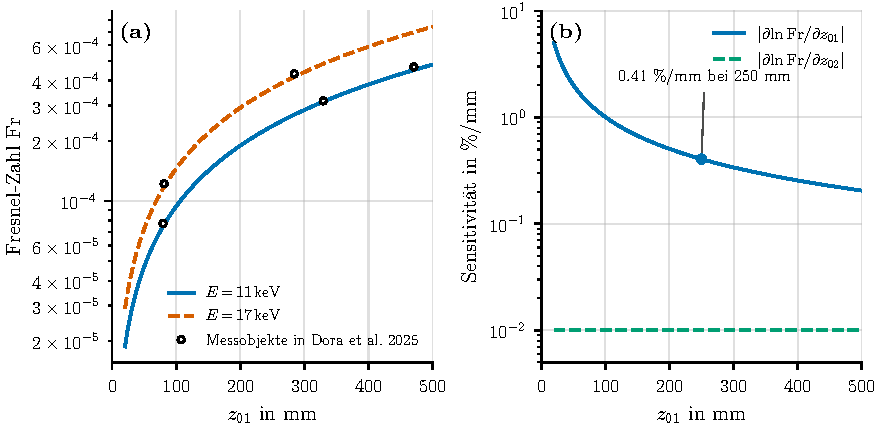
\includegraphics[width=\textwidth]{figures/grundlagen/sensitivitaet_z01}
  \caption[Fresnel-Zahl und ihre Sensitivität gegenüber $\zOne$ und $\zTwo$]{%
    (a)~Fresnel-Zahl $\Fr$ nach \cref{eq:grundlagen:fresnelzahl} als Funktion
    von $\zOne$ für die P05-Standardgeometrie ($\zTwo = \qty{20}{\metre}$,
    $\dx = \qty{6.5}{\micro\metre}$) bei \qty{11}{\kilo\electronvolt} und
    \qty{17}{\kilo\electronvolt}; die Kreise markieren die Geometrien der fünf
    Messobjekte aus \cite{dora2025autofocus} (Tab.~2 dort; $\Fr$ hier mit
    \cref{eq:grundlagen:fresnelzahl} berechnet). (b)~Logarithmische
    Sensitivitäten $\abs{\partial\ln\Fr/\partial\zOne}$ und
    $\abs{\partial\ln\Fr/\partial\zTwo}$ nach
    \cref{eq:grundlagen:sensitivitaet} in Prozent pro Millimeter: Ein Millimeter
    in $\zOne$ wirkt bei $\zOne = \qty{250}{\milli\metre}$ etwa vierzigmal
    stärker auf $\Fr$ als ein Millimeter in $\zTwo$.}
  \label{fig:grundlagen:sensitivitaet}
\end{figure}

% ---------------------------------------------------------------------------
\begin{figure}[tb]
  \centering
  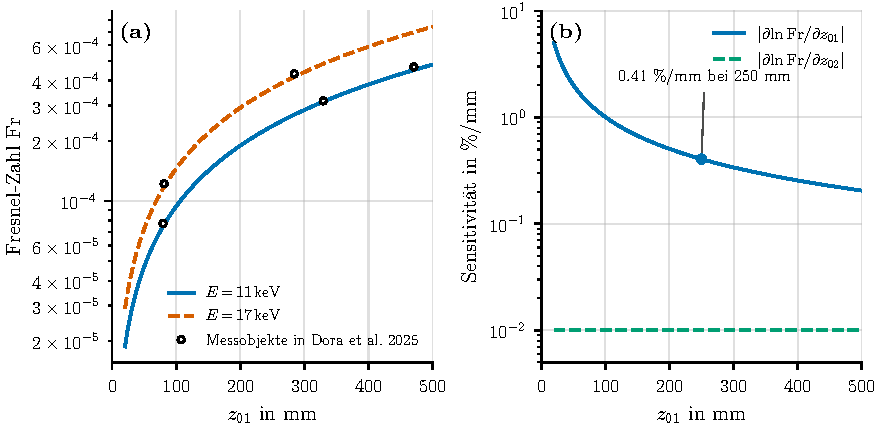
\includegraphics[width=\textwidth]{figures/grundlagen/sensitivitaet_z01}
  \caption[Fresnel-Zahl und ihre Sensitivität gegenüber $\zOne$ und $\zTwo$]{%
    (a)~Fresnel-Zahl $\Fr$ nach \cref{eq:grundlagen:fresnelzahl} als Funktion
    von $\zOne$ für die P05-Standardgeometrie ($\zTwo = \qty{20}{\metre}$,
    $\dx = \qty{6.5}{\micro\metre}$) bei \qty{11}{\kilo\electronvolt} und
    \qty{17}{\kilo\electronvolt}; die Kreise markieren die Geometrien der fünf
    Messobjekte aus \cite{dora2025autofocus} (Tab.~2 dort; $\Fr$ hier mit
    \cref{eq:grundlagen:fresnelzahl} berechnet). (b)~Logarithmische
    Sensitivitäten $\abs{\partial\ln\Fr/\partial\zOne}$ und
    $\abs{\partial\ln\Fr/\partial\zTwo}$ nach
    \cref{eq:grundlagen:sensitivitaet} in Prozent pro Millimeter: Ein Millimeter
    in $\zOne$ wirkt bei $\zOne = \qty{250}{\milli\metre}$ etwa vierzigmal
    stärker auf $\Fr$ als ein Millimeter in $\zTwo$.}
  \label{fig:grundlagen:sensitivitaet}
\end{figure}

% ---------------------------------------------------------------------------
\begin{figure}[tb]
  \centering
  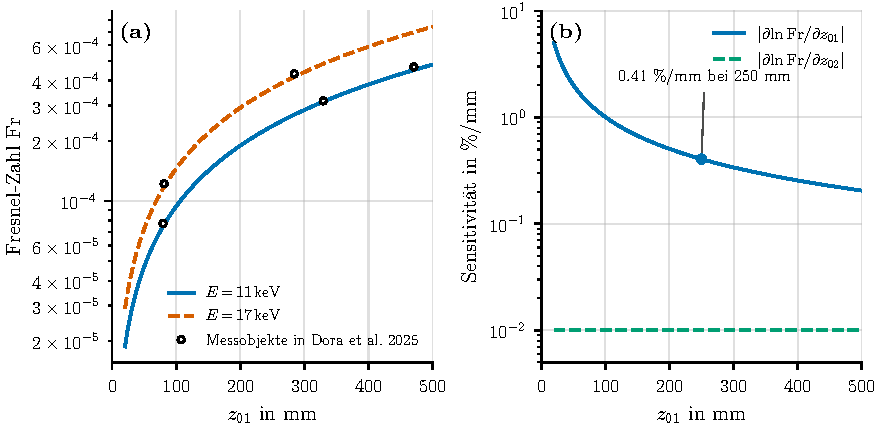
\includegraphics[width=\textwidth]{figures/grundlagen/sensitivitaet_z01}
  \caption[Fresnel-Zahl und ihre Sensitivität gegenüber $\zOne$ und $\zTwo$]{%
    (a)~Fresnel-Zahl $\Fr$ nach \cref{eq:grundlagen:fresnelzahl} als Funktion
    von $\zOne$ für die P05-Standardgeometrie ($\zTwo = \qty{20}{\metre}$,
    $\dx = \qty{6.5}{\micro\metre}$) bei \qty{11}{\kilo\electronvolt} und
    \qty{17}{\kilo\electronvolt}; die Kreise markieren die Geometrien der fünf
    Messobjekte aus \cite{dora2025autofocus} (Tab.~2 dort; $\Fr$ hier mit
    \cref{eq:grundlagen:fresnelzahl} berechnet). (b)~Logarithmische
    Sensitivitäten $\abs{\partial\ln\Fr/\partial\zOne}$ und
    $\abs{\partial\ln\Fr/\partial\zTwo}$ nach
    \cref{eq:grundlagen:sensitivitaet} in Prozent pro Millimeter: Ein Millimeter
    in $\zOne$ wirkt bei $\zOne = \qty{250}{\milli\metre}$ etwa vierzigmal
    stärker auf $\Fr$ als ein Millimeter in $\zTwo$.}
  \label{fig:grundlagen:sensitivitaet}
\end{figure}

% ---------------------------------------------------------------------------
\begin{figure}[tb]
  \centering
  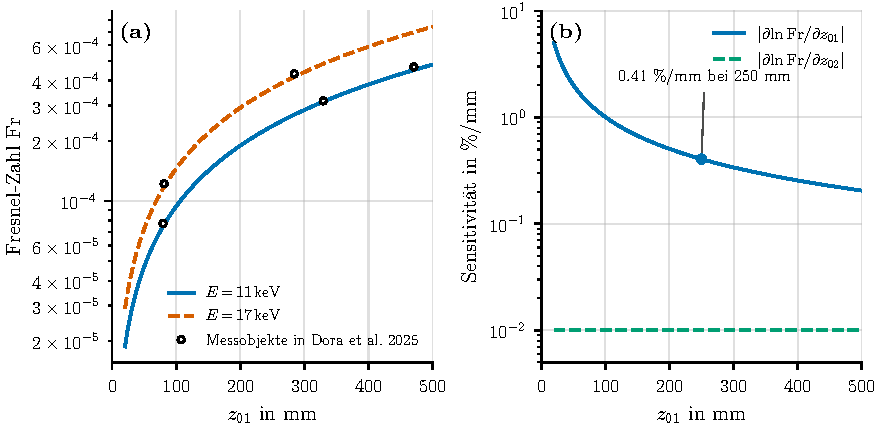
\includegraphics[width=\textwidth]{figures/grundlagen/sensitivitaet_z01}
  \caption[Fresnel-Zahl und ihre Sensitivität gegenüber $\zOne$ und $\zTwo$]{%
    (a)~Fresnel-Zahl $\Fr$ nach \cref{eq:grundlagen:fresnelzahl} als Funktion
    von $\zOne$ für die P05-Standardgeometrie ($\zTwo = \qty{20}{\metre}$,
    $\dx = \qty{6.5}{\micro\metre}$) bei \qty{11}{\kilo\electronvolt} und
    \qty{17}{\kilo\electronvolt}; die Kreise markieren die Geometrien der fünf
    Messobjekte aus \cite{dora2025autofocus} (Tab.~2 dort; $\Fr$ hier mit
    \cref{eq:grundlagen:fresnelzahl} berechnet). (b)~Logarithmische
    Sensitivitäten $\abs{\partial\ln\Fr/\partial\zOne}$ und
    $\abs{\partial\ln\Fr/\partial\zTwo}$ nach
    \cref{eq:grundlagen:sensitivitaet} in Prozent pro Millimeter: Ein Millimeter
    in $\zOne$ wirkt bei $\zOne = \qty{250}{\milli\metre}$ etwa vierzigmal
    stärker auf $\Fr$ als ein Millimeter in $\zTwo$.}
  \label{fig:grundlagen:sensitivitaet}
\end{figure}
